% Replace exercise 23's PNG figure and its figure-explanation box.
% The final blank Contact No cell also has colspan="2" in the CURRENT HTML.
\begin{center}
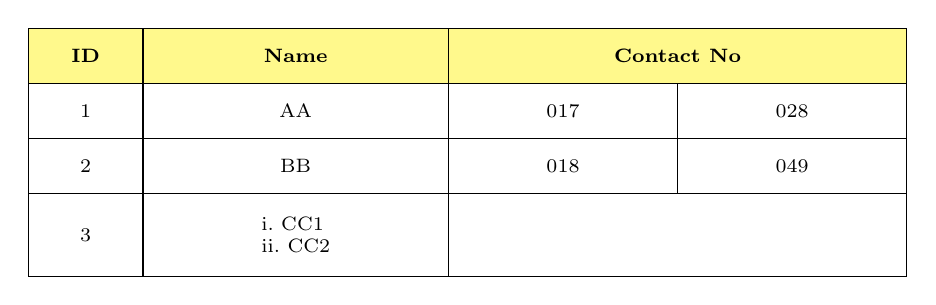
\begin{tikzpicture}[x=\linewidth,y=7mm,
  every node/.style={font=\scriptsize,align=center},line width=.5pt]
  \fill[yellow!45] (0,3.5) rectangle (.92,4.5);
  \draw (0,0) rectangle (.92,4.5);
  \draw (.12,0)--(.12,4.5) (.44,0)--(.44,4.5);
  \draw (.68,1.5)--(.68,3.5);
  \draw (0,1.5)--(.92,1.5) (0,2.5)--(.92,2.5) (0,3.5)--(.92,3.5);
  \node[font=\scriptsize\bfseries] at (.06,4) {ID};
  \node[font=\scriptsize\bfseries] at (.28,4) {Name};
  \node[font=\scriptsize\bfseries] at (.68,4) {Contact No};
  \node at (.06,3) {1}; \node at (.28,3) {AA};
  \node at (.56,3) {017}; \node at (.80,3) {028};
  \node at (.06,2) {2}; \node at (.28,2) {BB};
  \node at (.56,2) {018}; \node at (.80,2) {049};
  \node at (.06,.75) {3};
  \node[align=left] at (.28,.75) {i.\ CC1\\ii.\ CC2};
\end{tikzpicture}
\captionof{figure}{অনুশীলন 23: যোগাযোগের নম্বর}
\end{center}
\par\smallskip\textbf{চিত্র ব্যাখ্যা:} 
Contact No শিরোনাম দুটি নম্বরের কলাম জুড়ে আছে। শেষ সারিতেও \texttt{colspan="2"} দেওয়ায় ফাঁকা যোগাযোগের অংশটি একটি বিস্তৃত ঘর। Name ঘরের \texttt{ol type="i"} তালিকায় CC1 ও CC2-এর আগে i ও ii দেখা যায়।

